% sections/results.tex -- Results: validation on known orders, performance, new coefficients
\section{Results}
\label{sec:results}

The numbers of Secs.~\ref{sec:results-validation} and~\ref{sec:results-performance} come from the runs recorded in
the ledger (Sec.~\ref{sec:methods-ledger}), on nodes with NVIDIA H200 GPUs: device self-tests, comparisons of the GPU
and CPU code paths on identical random numbers, validation runs at two to five loops, replica ensembles,
measurements of throughput, tuning and scaling, and complete orders at four to seven loops in production mode.
Section~\ref{sec:results-new} gives the new coefficients, from eight to ten loops.

Unless stated otherwise, values refer to $N=1$, and $B_L$, $H_L$, $C_L$ are the per-order sums of
Eqs.~\eqref{eq:series} and~\eqref{eq:BHC}. Errors are one standard deviation of the Monte Carlo estimate. At two loops
we compare with the exact values of Eq.~\eqref{eq:exactsums}, $1/2$, $1/81$ and $1/12$ at $N=1$. From three loops on,
we compare with reference values derived from the $O(N)$
series of $\beta$, $\eta$ and $\nu$ of Ref.~\cite{Phi4tools2024}: we invert the Callan--Symanzik
relations~\eqref{eq:csrel} order by order~\check{S1} and propagate the quoted uncertainties of the series coefficients to first
order, adding their effects in absolute value, which is conservative. Agreement is measured by the pull $z$ of
Eq.~\eqref{eq:pull}.

%-----------------------------------------------------------------------------------------------------------------------
\subsection{Validation on known orders}
\label{sec:results-validation}

A computation of this kind can fail in three ways that a single run does not reveal: the integrands, or the code
that evaluates them, can be wrong; the error bars can be too small; and the round-off of the cancellations inside the
subtracted integrands can bias the means. Comparisons with known values test the first, but only as far as the error
bars are right, and round-off at the level that matters lies below the precision of any reference. We therefore test
the error bars and the round-off separately, without references, after establishing that runs on GPUs and on CPUs can
be pooled.

\paragraph{GPU against CPU.}
On identical random numbers the GPU and CPU code paths evaluate the same points and can differ only through the
device's mathematical library and the contraction of multiplications and additions (Sec.~\ref{sec:methods-kernel}).
Over the 13 configurations of the golden runs, 868 classes at three to six loops, the per-class means agree to within
0.59 units of the double-precision round-off scale of the per-sample terms, $\epsilon_{\rm mach}\sum|\text{terms}|$,
and the order sums to within $6\times10^{-10}$ standard deviations, on each device alone and with the work split over
all of them~\check{N2}; fused multiply-add contraction, which only the earliest runs used, stays within the same
bound. The hardware therefore adds nothing to the error budget, and runs are pooled whatever device produced them.

\paragraph{Known values.}
The two-loop sums reproduce their exact values, $B_2=1/2$, $H_2=1/81$ and $C_2=1/12$ at $N=1$, within their errors and
to relative uncertainties of a few $10^{-7}$ (Table~\ref{tab:validation})~\check{N3}.

\begin{table*}
\caption{\label{tab:validation}%
Per-order sums at $N=1$ compared with exact values ($L=2$) and with values derived from the
series of Ref.~\cite{Phi4tools2024} ($L\ge3$; uncertainties not shown are below $10^{-9}$ relative). The reference for
$C_7$ was derived in the same way. This work: every contribution of the ledger (validation runs with a
pilot of 65\,536 samples per class, production-mode runs of complete orders with a pilot of 16\,384 or 32\,768,
replicas; all with Neyman allocation by measured device time, within a fixed time box or up to a target uncertainty)
pooled class by class.
Classes: graphs with a non-vanishing subtracted integrand (twins were not merged). $z$: pull,
Eq.~(\ref{eq:pull}). Cost: the integrand evaluations of all its runs, in Tf (1~Tf $=10^{12}$ function evaluations), a
measure of the cost that does not depend on the hardware (Table~\ref{tab:cost}). Generated from the ledger~\checks{N3,N4,S2}.}
% generated/validation.tex -- body of Table tab:validation (per-order sums at N=1 against the references).
% WRITTEN BY series/tables.py (make -C ../series) from ledger/orders.json: do not edit by hand.
% This work: all contributions of the ledger pooled class by class. Reference: exact (L = 2) or derived from
% Phi4tools through the Callan-Symanzik relations (integrator/tools/refs.py); z = pull.
\begin{ruledtabular}
\begin{tabular}{lrlrlllr}
Sum & $L$ & Reference & Classes & This work & $\delta X/|X|$ & Cost [Tf] & $z$ \\
\hline
$B_L$ & 2 & $1/2$ & 1 & 0.50000006(33) & $6.7\times10^{-7}$ & 1.9 & $+0.18$ \\
 & 3 & 0.598603706 & 6 & 0.59860364(29) & $4.8\times10^{-7}$ & 18 & $-0.23$ \\
 & 4 & 0.967192687 & 19 & 0.96719250(71) & $7.3\times10^{-7}$ & 23 & $-0.26$ \\
 & 5 & 1.89652536(49) & 96 & 1.8965261(12) & $6.2\times10^{-7}$ & 77 & $+0.57$ \\
 & 6 & 4.3006836(49) & 502 & 4.3006914(59) & $1.4\times10^{-6}$ & 33 & $+1.02$ \\
 & 7 & 10.917594(45) & 3150 & 10.917628(31) & $2.8\times10^{-6}$ & 17 & $+0.63$ \\
\hline
$H_L$ & 2 & $1/81$ & 1 & 0.0123456808(24) & $2.0\times10^{-7}$ & 2.7 & $+0.75$ \\
 & 3 & $-0.001542750058$ & 1 & $-0.0015427487(12)$ & $8.0\times10^{-7}$ & 34 & $+1.09$ \\
 & 4 & 0.004699104918 & 4 & 0.0046991056(34) & $7.1\times10^{-7}$ & 15 & $+0.21$ \\
 & 5 & 0.002443913(10) & 11 & 0.002443919(10) & $4.2\times10^{-6}$ & 8 & $+0.37$ \\
 & 6 & 0.008020564(89) & 50 & 0.008020530(36) & $4.5\times10^{-6}$ & 4.3 & $-0.36$ \\
 & 7 & 0.01454955(80) & 209 & 0.014550034(71) & $4.9\times10^{-6}$ & 9.7 & $+0.60$ \\
\hline
$C_L$ & 2 & $1/12$ & 1 & 0.083333395(56) & $6.8\times10^{-7}$ & 1.5 & $+1.09$ \\
 & 3 & 0.07785997192 & 2 & 0.077860025(39) & $5.0\times10^{-7}$ & 9.7 & $+1.35$ \\
 & 4 & 0.1006770275 & 5 & 0.100677024(76) & $7.6\times10^{-7}$ & 24 & $-0.04$ \\
 & 5 & 0.170551919(82) & 16 & 0.17055175(21) & $1.2\times10^{-6}$ & 24 & $-0.77$ \\
 & 6 & 0.34591073(86) & 62 & 0.34591043(98) & $2.8\times10^{-6}$ & 9.8 & $-0.23$ \\
 & 7 & 0.801121(11) & 265 & 0.8011143(39) & $4.9\times10^{-6}$ & 6.5 & $-0.53$ \\
\end{tabular}
\end{ruledtabular}
% body written by `make -C ../series`
\end{table*}

All \valncmp\ comparisons at three to seven loops in Table~\ref{tab:validation} lie within \valzmax\ standard
deviations, with $\chi^2=\valchisq$ for \valncmp\ values ($p=\valpval$)~\check{N4}. The reference errors, added
linearly over the coefficients of the $N$ polynomials of Ref.~\cite{Phi4tools2024}, are conservative, and the pulls are
correspondingly small. The complete seven-loop orders
$B_7$ ($\beta$ at $\ubar^{8}$, \nclBseven\ classes), $H_7$ ($\eta$ at $\ubar^{7}$, \nclHseven) and $C_7$ ($\nu$ at
$\ubar^{7}$, \nclCseven) reach relative uncertainties of \relBseven, \relHseven\ and \relCseven, below those of the
references by factors of about \precBseven, \precHseven\ and \precCseven; at six loops, with the computing time we
allocated, the precision of the references is matched (ratios of their uncertainty to ours of \precBsix,
\precHsix\ and \precCsix). The four-loop references are known to $2\times10^{-11}$ or better, which makes the
four-loop sums the most stringent test of a bias common to all classes: with relative uncertainties of at most
\fourrelmax, $B_4$, $H_4$ and $C_4$ deviate jointly from the references by \fourjointdev, so any common bias is below
\fourbiasbound\ at 95\% confidence, and that of $H_4$ alone below \hfourbiasbound.

Every class carries its $O(N)$ weight polynomial, so the same runs give the sums at any $N$, with errors that follow
from the class errors without further assumptions. Recombined at $N=0$, 2, 3 and 4, the same \valncmp\ comparisons
give $\chi^2$ between \valNchisqmin\ and \valNchisqmax\ and no pull larger than \valNzmax\ in
magnitude~\checks{N4,S2}; they come from the same samples as those at $N=1$ and are correlated with them.

\paragraph{Error bars.}
The value of a class is the mean of its weights, and its error the standard deviation of the weights divided by the
square root of their number (Sec.~\ref{sec:methods-estimators}). The mean is unbiased whatever the distribution of the
weights, but the error is only as reliable as the sample variance, and the subtractions make that the delicate part.
Near a face of the parameter space where the lines of a renormalization part, a two- or four-point subgraph, shrink to
zero, the subtracted integrand stays finite only through cancellations between its forest terms, and the tropical
density, which keeps the variance finite (Sec.~\ref{sec:methods-tropical}), follows it there only approximately. The
weights of classes with renormalization parts therefore have heavy tails: at seven loops the kurtosis reaches
\kurtmaxseven\ (a class of \kurtmaxsevenorder) and the largest weight is up to \wmaxmaxseven\ times the class mean (a
class of \wmaxmaxsevenorder). With such tails the sample variance converges slowly, and the rare large weights that
carry part of the variance may not yet have been drawn: in a short run the quoted error of such a class is more often
too small than too large. Comparisons with references cannot detect this at the precision we reach, so we test the
error bars directly, by repeating computations with independent seeds and comparing the scatter of the results with
their quoted errors.

We made this test where it is most likely to fail, in short runs: eight independent replicas of each of $B_6$, $H_6$,
$C_6$, $B_7$, $H_7$ and $C_7$, each sampling for four to eight minutes on one GPU, with medians of $10^{7}$ to $10^{9}$
samples per class. The replicas scatter as their quoted errors say: for the order sums $\chi^2=31.6$ for 42 degrees of
freedom ($p=0.88$), and class by class, over the 29\,666 degrees of freedom of the classes sampled in every replica,
$\chi^2/{\rm dof}=1.003$ ($p=0.36$); the classes that carry half of the variance of each order, the heavy-tailed ones
among them, give $\chi^2/{\rm dof}$ between 0.93 and 1.20~\check{N7}. A second test needs no reference either, and
grows with every run: each run merged into the ledger is compared, class by class, with the pool of the runs before
it (Sec.~\ref{sec:methods-ledger}). Over the \mergeruns\ runs so compared, in \mergeorders\ orders from \mergeLmin\
to \mergeLmax\ loops, the per-class $\chi^2$ is \mergechisq\ for \mergedof\ degrees of freedom
($\chi^2/{\rm dof}=\mergeratio$); the deviations of the runs' $\chi^2$ from their expectations, in units of their
standard deviations, have mean \mergezmean\ and spread \mergezsd, as they should for correct errors; and the order
sums on the common classes give $\chi^2=\mergesumchisq$ for \mergesumn\ runs
($p=\mergesump$)~\checks{N5,S2}.

Beyond seven loops the tails are heavier: the kurtosis reaches \kurtmaxhigh\ (a class of \kurtmaxhighorder) and the
largest weight \wmaxmaxhigh\ times the class mean (a class of \wmaxmaxhighorder). At eight loops the independent runs
of $B_8$ and $H_8$ scatter as their errors say (Table~\ref{tab:newsums}); the ten runs of $B_7$ scatter less than
theirs, which suggests conservative rather than optimistic errors, and we quote the pooled errors without rescaling.
For the single runs of $C_8$, $H_9$ and $C_9$, and for the slices of $B_9$, $B_{10}$, $H_{10}$ and $C_{10}$, no replica
test exists: their errors rest on the within-run statistics, and the runs driven to a target uncertainty stopped on
their own error estimates, a data-dependent rule whose effect we have not quantified.

\paragraph{Round-off in the subtractions.}
The forest formula, Eq.~\eqref{eq:integrand}, writes a subtracted integrand as a sum of terms, the bare integrand and
one subtraction for each forest of renormalization parts, that diverge separately on the faces where the lines of a
part shrink; only their sum is integrable. Close to such a face the terms are large and nearly cancel, and the
double-precision sum carries an absolute error of the order of $\epsilon_{\rm mach}\sum|\text{terms}|$
(Sec.~\ref{sec:methods-rng}). Unlike the sampling error, this error does not decrease with more samples and is not part
of the quoted errors; with a preferred sign it would bias the class means, below the precision of any reference. It
grows with the number of renormalization parts, hence with the order, and with the number of samples, which come ever
closer to the faces. Among the four classes of $H_4$, for instance, the only one with a two-point part, a sunset, has a
single-sample round-off scale of up to $6\times10^{-4}$ of its per-sample standard deviation, against about
$10^{-13}$ in the other three.

Every run records, for each class, the largest round-off scale of a single sample and its root mean square over the
samples, in units of the per-sample standard deviation. At seven loops the single-sample scale exceeds $10^{-3}$ in
\rmaxcountBseven\ of the \nclBseven\ classes of $B_7$ (largest \rmaxmaxBseven), \rmaxcountHseven\ of the \nclHseven\ of
$H_7$ and \rmaxcountCseven\ of the \nclCseven\ of $C_7$. The rms scale, which is what could shift a mean, stays far
smaller: through seven loops it is at most \rmsmaxlow\ of the per-sample spread, and at eight to ten loops it exceeds
$10^{-3}$ in \rmscounthigh\ classes, up to \rmsmaxhigh\ in a class of \rmsmaxhighorder. If every sample of every class
were shifted coherently by its rms scale, the order sums would move by at most \rcohmax\ of their statistical errors,
at any order from four to ten loops (the largest for \rcohmaxorder).

Since the scales are estimates, we also measured the round-off itself where it is largest: the same $2\times10^{5}$
sample points of each of 55 classes, the 43 most exposed of $B_8$, $H_8$, $C_8$, $H_9$, $C_9$ and $C_{10}$ and two
controls per order at six and seven loops, were evaluated in double and in extended (64-bit-mantissa) precision on the
CPU ($B_9$, $B_{10}$ and $H_{10}$, completed later, are covered by the bound above). The measured rms round-off is
typically 25 times below the scale (median), but in two classes of $C_{10}$ it reaches $0.1$ and $1.0$ of the
per-sample spread; there it adds to the sample variance, which the quoted errors include. No class shows a significant
mean difference between the two precisions (the largest is $1.9$ standard errors among the 55), and summed over the
classes of an order the possible bias is at most $4\times10^{-6}$ of the order's statistical error~\check{N6}. Since
the GPU and CPU code paths agree on identical samples to a fraction of the round-off scale~\check{N2}, the conclusion
carries over to the GPU runs. No run produced a non-finite weight.

%-----------------------------------------------------------------------------------------------------------------------
\subsection{Performance}
\label{sec:results-performance}

\paragraph{Hardware and kernel.}
The bulk of the numerical evaluations of this work were run on computing nodes with NVIDIA H200 GPUs and Intel Xeon
Platinum 8568Y+ host CPUs. Each H200 GPU has compute capability~9.0, 132 streaming multiprocessors at 1.98~GHz, 140~GiB of memory with ECC enabled,
and a double-precision rate of half the single-precision rate; the host CPUs also build the classes. The code was compiled with CUDA~12.1 for sm\_90. The
integration kernel uses 110 registers per thread and 1104 bytes of stack, so four blocks of 128 threads fit on a
multiprocessor, and the grid has 528 blocks per device. Launches are sized to fill whole waves of the grid, with mean
fill factors of 0.99--1.00. In the production-mode runs the devices were busy
96--99\% of the wall time. The host builds the classes. For the \nclBseven\ classes of $B_7$ this takes
\costcpus{b7}~s summed over classes.

\begin{table}
\caption{\label{tab:throughput}%
Throughput with equal allocation over the classes of an order: samples per second summed over four NVIDIA H200
GPUs, and mean and maximum over the classes of the
device time per sample on one GPU. $b$, $h$, $c$: the subtracted integrands of $B_L$, $H_L$, $C_L$.
int4: the four-point integrands of the intermediate scheme of Ref.~\cite{Phi4tools2024}. bare4: unsubtracted
four-point integrands.}
\begin{ruledtabular}
\begin{tabular}{lrrll}
Kind & $L$ & Classes & Rate [$10^9$/s] & ns/sample \\
\hline
$b$    & 4 & 19  & 2.42  & 1.65 / 2.25 \\
       & 5 & 96  & 1.22  & 3.29 / 6.05 \\
       & 6 & 502 & 0.652 & 6.13 / 15.5 \\
$h$    & 4 & 4   & 2.00  & 2.00 / 2.51 \\
       & 5 & 11  & 0.889 & 4.50 / 6.45 \\
       & 6 & 50  & 0.431 & 9.25 / 17.0 \\
$c$    & 4 & 5   & 0.997 & 4.01 / 5.16 \\
       & 5 & 16  & 0.394 & 10.2 / 17.3 \\
       & 6 & 62  & 0.162 & 24.5 / 54.3 \\
int4   & 4 & 27  & 7.00 & 0.571 / 0.804 \\
       & 5 & 129 & 4.58 & 0.874 / 1.61 \\
       & 6 & 660 & 3.06 & 1.31 / 2.36 \\
bare4  & 4 & 23  & 7.38 & 0.542 / 0.574 \\
       & 5 & 105 & 4.92 & 0.812 / 0.844 \\
\end{tabular}
\end{ruledtabular}
\end{table}

\paragraph{Throughput.}
Table~\ref{tab:throughput} gives the sampling rates. For the subtracted integrands the cost per sample about doubles
with every loop: 1.65, 3.29, 6.13~ns per sample and GPU for $b$ at four, five and six loops, and
4.0, 10.2, 24.5~ns for $c$. At the same orders, a subtracted four-point integrand costs
2.9, 3.8 and 4.7 times as much per sample as the corresponding intermediate-scheme integrand. In the
seven-loop production-mode runs, with Neyman allocation, the four GPUs drew $7.3\times10^{8}$,
$3.1\times10^{8}$ and $1.1\times10^{8}$ samples per second for $B_7$, $H_7$ and $C_7$.

\paragraph{Tuning.}
The default kernel is limited by registers to a quarter of the maximum thread occupancy. Capping the registers so that
six or eight blocks fit on a multiprocessor raises the throughput of the five-loop $b$ and $c$ kernels by 20--22\% and
30--33\%. This holds even though the six- and eight-block builds spill
96 and 232~bytes per thread to local memory. The deviations from the CPU do not change. The production-mode runs
of this section used the default build, so their costs would drop by roughly a quarter if the five-loop gains carry
over. At five loops, disabling FMA contraction (the default from version 0.4.0) costs 1\% of throughput and brings the
GPU about five times closer to the CPU, which is compiled without contraction: the worst per-class deviation from the
CPU on identical random numbers moves from 0.072 to 0.015.

\paragraph{Scaling.}
Classes are independent: each GPU draws units of work from a shared queue, and the host only merges per-class
accumulators. On one, two and four GPUs the five-loop
$B_5$ run drew $3.03$, $6.01$ and $12.1\times10^{8}$ samples per second of wall time, a parallel
efficiency of 99\% at two and at four GPUs. Beyond one node no communication is needed: the larger orders were
split into slices of their lists, each run as an independent job on one or four GPUs and pooled in the ledger
(Sec.~\ref{sec:results-new}).

\paragraph{Cost per decade of precision.}
For a Monte Carlo estimate the relative uncertainty after a device time $T_{\rm dev}$ (summed over GPUs) is
$\delta X/|X|=\rho_\tau\,T_{\rm dev}^{-1/2}$, with $\rho_\tau$ of Eq.~\eqref{eq:rho} under optimal allocation. Each
decade of precision therefore costs a factor of 100 in time. We take the realized value
$\rho_\tau=(\delta X/|X|)\sqrt{T_{\rm dev}}$ of each order, with $\delta X/|X|$ its uncertainty from all its runs pooled
and $T_{\rm dev}$ the device time of those runs; for a single production-mode run it is within about 1\% of the value
predicted by Eq.~\eqref{eq:rho}. Table~\ref{tab:cost} and Fig.~\ref{fig:cost} give the device time
$T_{\rm dev}(10^{-5})=(\rho_\tau/10^{-5})^2$ needed for a relative uncertainty of $10^{-5}$. From one order to the next,
$\rho_\tau^2$ grows by \costratios{b} for $B_L$ (from \costratiorange{b} loops) and by \costratios{c} for $C_L$ (from
\costratiorange{c}): the growth factors fall from four to six at low orders to about three from seven loops on. For
$H_L$ the sequence (\costratios{h}) is irregular at low orders, because $H_5$ has an unusually large per-sample
spread. At seven loops a relative uncertainty of $10^{-5}$ costs \costTm{b7}, \costTm{h7} and \costTm{c7} GPU hours
for $B_7$, $H_7$ and $C_7$. Matching the precision of the reference value of $B_6$ ($\costrefbsix\times10^{-6}$) would
take \costmatchbsix\ GPU hours, about \costmatchbsixfour~h on four GPUs.

\begin{table}
\caption{\label{tab:cost}%
Cost of the sums on NVIDIA H200 GPUs. $\delta X/|X|$: the relative uncertainty of the sum, all
its runs pooled. $\rho_\tau=(\delta X/|X|)\sqrt{T_{\rm dev}}$, with $T_{\rm dev}$ the device time of those runs summed
over their GPUs, does not depend on how long they ran; $T_{\rm dev}(10^{-5})=\rho_\tau^2/10^{-10}$ is the device time
for a relative uncertainty of $10^{-5}$, in GPU hours, the quantity to compare between orders (Fig.~\ref{fig:cost}).
$\rho_n=(\delta X/|X|)\sqrt{n}$ and $n(10^{-5})=\rho_n^2/10^{-10}$ are the same with $n$, the number of integrand
evaluations of those runs, in place of the device time, in Tf ($10^{12}$ evaluations): they do not depend on the hardware.
The numbers of classes are in Tables~\ref{tab:validation} and~\ref{tab:newsums}. Generated from the
ledger~\check{S2}.}
\footnotesize
\begin{ruledtabular}
\begin{tabular}{lrrrrrr}
Sum & $L$ & $\delta X/|X|$ & $\rho_\tau$ & $T_{\rm dev}(10^{-5})$ & $\rho_n$ & $n(10^{-5})$ \\
    &     & [$10^{-5}$] & [$10^{-4}\,$s$^{1/2}$] & [h] & & [Tf] \\
\hline
\costtablerows% written by series/costfig.py from the ledger
\end{tabular}
\end{ruledtabular}
\end{table}

\begin{figure}
\centering
\ifdefined\pgfplotsversion
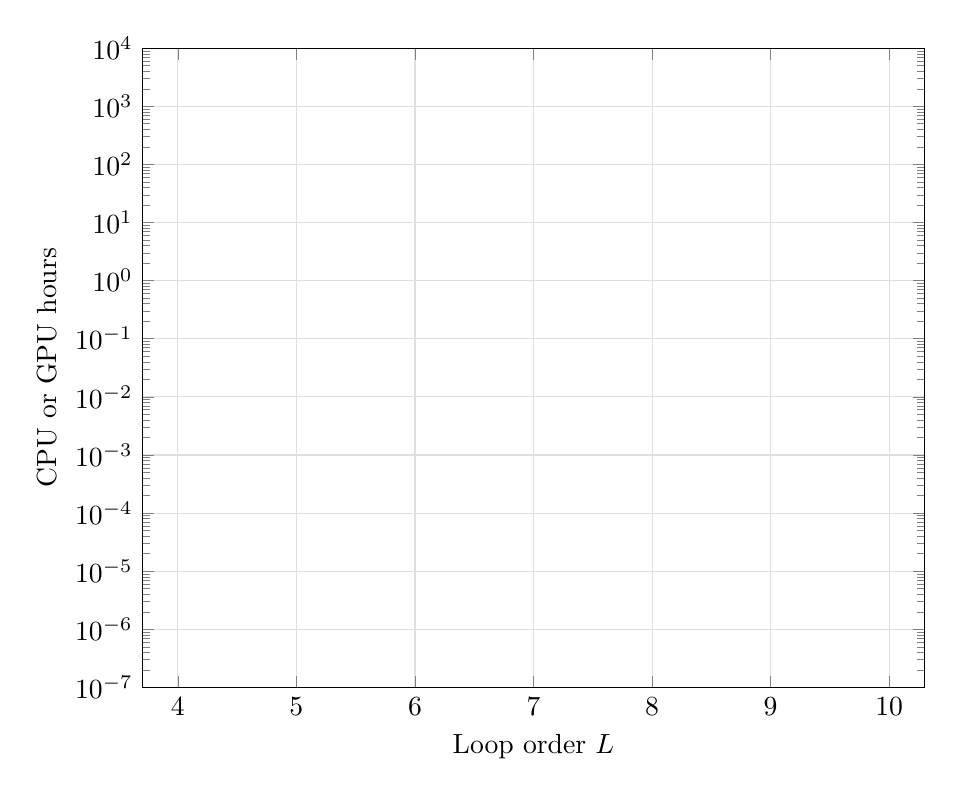
\begin{tikzpicture}
\begin{semilogyaxis}[
  width=0.95\columnwidth, height=0.8\columnwidth,
  xlabel={Loop order $L$}, ylabel={CPU or GPU hours},
  xtick={4,5,6,7,8,9,10}, xmin=3.7, xmax=10.3, ymin=1e-7, ymax=1e4,
  legend pos=south east, legend columns=2, legend cell align=left, legend style={font=\scriptsize},
  grid=major, grid style={gray!25}]
\costcurves
\end{semilogyaxis}
\end{tikzpicture}
\else
(This figure needs the \texttt{pgfplots} package.)
\fi
\caption{\label{fig:cost}%
The two costs of an order: the CPU time of the class build (dashed; the sum over the classes of the single-thread
build times recorded in the ledger, in hours of one core of an Intel Xeon Platinum 8568Y+) and the GPU time of the sampling to a relative uncertainty
of $10^{-5}$ (solid; the measured $T_{\rm dev}(10^{-5})$ of Table~\ref{tab:cost}, in hours of one NVIDIA H200 GPU,
which scales as the inverse square of the target uncertainty). From seven loops on the sampling grows by a factor
of \costgrowthrange\ per loop, the build by \cpugrowthrange, since the
sector table of a class spans the $2^\ell$ subsets of its lines and the minimum over its terms grows with them. For
$H_L$ and $C_L$ the sampling dominates through nine loops and the build at ten; for $B_L$, whose classes are many and
small, the build dominates from nine loops on. Generated from the ledger~\check{S2}.}
\end{figure}

\begin{figure*}
\centering
\ifdefined\pgfplotsversion
\definecolor{colL6}{named}{blue}\definecolor{colL7}{named}{red}\colorlet{colL8}{green!55!black}
\definecolor{colL9}{named}{orange}\definecolor{colL10}{named}{violet}
\pgfplotsset{costhist/.style={scale only axis, width=0.285\textwidth, height=0.22\textwidth, xlabel={$\log_{10}\kappa_G$},
  xmin=-11.5, xmax=-3, ymin=0, ymax=36, ytick={0,10,20,30}, grid=major, grid style={gray!25},
  legend cell align=left,
  legend style={at={(0.02,1)}, anchor=north west, yshift=-0.4mm, font=\tiny, draw=none, fill=none, row sep=-1.2pt,
    inner sep=1pt, nodes={inner ysep=0.4pt}},
  legend image code/.code={\draw[#1, thick] (0cm,0cm) -- (0.3cm,0cm);},
  title style={font=\small, yshift=-1ex}}}
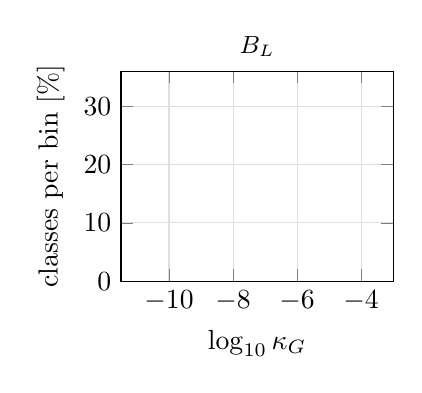
\begin{tikzpicture}
\begin{axis}[costhist, title={$B_L$}, ylabel={classes per bin [\%]}]
\costhistB
\end{axis}
\end{tikzpicture}\hfill
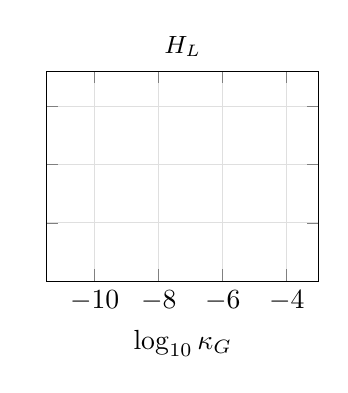
\begin{tikzpicture}
\begin{axis}[costhist, title={$H_L$}, yticklabels={}]
\costhistH
\end{axis}
\end{tikzpicture}\hfill
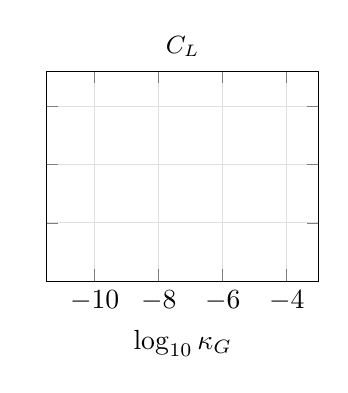
\begin{tikzpicture}
\begin{axis}[costhist, title={$C_L$}, yticklabels={}]
\costhistC
\end{axis}
\end{tikzpicture}
\else
(This figure needs the \texttt{pgfplots} package.)
\fi
\caption{\label{fig:costhist}%
Distribution over the classes of an order of the Neyman cost weight $\kappa_G = |a_G|\sigma_G\sqrt{\tau_G}/|X_L|$,
where $a_G\sigma_G$ is the standard deviation per sample of the weighted contribution of class $G$, $\tau_G$ its device
time per sample and $X_L$ the order sum: the device time that brings $X_L$ to the relative uncertainty $\epsilon$ is
$T(\epsilon) = (\sum_G\kappa_G)^2/\epsilon^2$, and class $G$ receives the fraction $\kappa_G/\sum_{G'}\kappa_{G'}$ of it
[Eq.~\eqref{eq:rho}]. Each histogram is normalized to the number of classes of its order (in the legends); the bins are a
quarter of a decade wide, and $\kappa_G$ is in $\sqrt{\rm s}$ of H200 time, from the pooled per-class statistics. From one order to the next the
distributions move to the left by about \kappashift\ decades while the number of classes grows by a factor of
\graphgrowthrange, so that $\sum_G\kappa_G$ grows only by a factor of \kappagrowthrange\ per loop. The resulting $T(10^{-5})$, $\costT{b8}$,
$\costT{h9}$ and $\costT{c9}$ GPU hours for $B_8$, $H_9$ and $C_9$, reproduces the measured
times of Table~\ref{tab:cost} and Fig.~\ref{fig:cost} to within \costkappadev\%. Generated from the ledger~\check{S2}.}
\end{figure*}


\paragraph{Scaling with the loop order.}
Figure~\ref{fig:cost} shows that the two costs of an order grow in different ways. The CPU time of the class build
curves upwards on the logarithmic scale: its growth per loop increases with the order, to a factor of \cpugrowthrange\
from seven loops on---the superexponential growth expected of a number of graphs that grows factorially times a sector
table that doubles with every line. The GPU time of the sampling curves the other way: its growth per loop decreases
with the order and settles, from seven loops on, at a factor of about \costgrowth{b} for $B_L$, \costgrowth{h} for
$H_L$ and \costgrowth{c} for $C_L$, so that the device time for a fixed relative uncertainty grows at most geometrically,
not factorially as the number of graphs does (from seven to ten loops the lists grow by factors of 6.7 to 8.1 per loop
for $\Gamma^{(4)}$ and 5.1 to 6.5 for $\Gamma^{(2)}$). Counted in
integrand evaluations, which do not depend on the hardware, the growth is slower still: the evaluations needed for a
relative uncertainty of $10^{-5}$ grow by a factor of \evalgrowthrange\ per loop (Table~\ref{tab:cost}), and the rest of
the growth of the device time is the growing cost of one evaluation. Two effects combine. The cost of a sample grows slowly,
because a class of $\ell$ lines costs a spanning-tree pass and an $L\times L$ factorization per atom and the number of
atoms per class stays small after the pruning, 19 on average at six loops and 26 at seven
(Sec.~\ref{sec:methods-construction}); and
the relative variance of an order grows slowly, because the sampling density follows the forest-subtracted
integrand sector by sector, so that the cancellations between forest terms happen inside each sample.
Figure~\ref{fig:costhist} shows the second effect graph by graph: under the Neyman allocation of Eq.~\eqref{eq:rho}
the device time of an order is $(\sum_G\kappa_G)^2/\epsilon^2$, with $\kappa_G$ as in Fig.~\ref{fig:costhist}, and
reconstructing it from the ledger reproduces the measured times to within \costkappadev\%. The distribution of
$\kappa_G$ is broad, about one decade wide, and the effort is not concentrated in a few classes: at every order
\costninetyrange\% of the classes are needed to account for 90\% of the cost. The median
$\kappa_G$ falls by about \kappashift\ decades per loop, because the typical graph shrinks faster than the
order sum grows, while the number of classes grows by a factor of \graphgrowthrange, so that $\sum_G\kappa_G$ grows by
\kappagrowthrange\ per loop and the cost by its square. At this rate
the sums of the tenth order cost up to a few hundred GPU hours at $10^{-5}$ (from $\costTm{b9}$ for $B_9$ to
$\costTm{c10}$ for $C_{10}$), and the limiting factor becomes the
generation and the symbolic preparation of the graphs rather than the sampling. Figure~\ref{fig:cost} shows the
crossing: the class build, which is dominated by the sector table over the $2^\ell$ subsets of lines, took
$\costcpu{c9}$ CPU hours for $C_9$ against $\costTm{c9}$ GPU hours of sampling, but grows by a
factor of \cpugrowthrange\ per loop and increasingly so with the order, so that at ten loops it exceeds the sampling
and is run
on CPU nodes, once per class, into the class cache of Sec.~\ref{sec:methods-construction}. For the three sums of the
tenth order, $B_9$, $H_{10}$ and $C_{10}$, the build took \costtenthcpu\ core-hours, against \costtenthgpu\ GPU hours
of sampling to the precisions of Table~\ref{tab:newsums}; in node-hours, with 32 cores per CPU node and the eight H200 GPUs of a GPU node, that is \costtenthnodecpu\ against \costtenthnodegpu.


\paragraph{Route A against route B.}
With the integrator of Sec.~\ref{sec:methods-numerics} the per-sample relative standard deviation of the order sum,
$\rho$ of Eq.~\eqref{eq:rho}, is 3.38 and 5.22 for $B_4$ and $B_5$, and 2.79 and 11.6 for $H_4$ and $H_5$, against 19.2,
40.5, 13.8 and 101 for the intermediate-scheme input of route B alone at the same order: the subtracted integrands
need 32, 60, 24 and 76 times fewer samples or, as each sample costs 2.4 to 3.9 times more on the CPU, 14, 22, 8 and 19
times less work at equal instruction count. These gains are lower bounds, since the route-B figures include only the
highest-order input, and they grow with the loop order. On the GPUs, where a subtracted four-point sample costs 2.9 and
3.8 times more at four and five loops (Table~\ref{tab:throughput}), the GPU time for $B_4$ and $B_5$ drops by factors of
about 11 and 16. At the ninth and tenth orders the route-B runs of Table~\ref{tab:routes}, \routeBhours\ GPU hours
in all, give coefficients whose uncertainties are \routeBratiomin\ to \routeBratiomax\ times those of route A.


\begin{table*}
\caption{\label{tab:effort}%
Computing effort of complete fixed-dimension computations. The entries are not like for like: they differ in the
quantities computed (individual graphs in Refs.~\cite{NMB1977,Phi4tools2024}, complete per-order sums here), in the
nature of the uncertainty (deterministic convergence estimates, VEGAS errors per graph, statistical errors per order),
and in the hardware. This work: per loop order, the sums computed and their classes, the device time for a relative
uncertainty of $10^{-5}$ of each sum (GPU h, Table~\ref{tab:cost}) and, from eight loops on, the CPU time of the class
construction (CPU h). The row of this work is generated from the ledger~\check{S2}.}
\begin{ruledtabular}
\raggedcolumns
\begin{tabular}{p{2.2cm}p{4.7cm}p{2.35cm}p{4.7cm}p{2.35cm}}
Computation & Quantities & Hardware & Time & Uncertainty \\
\hline
Nickel et al.~\cite{NMB1977,BNM1978} & $\Gamma^{(2)}$, $\Gamma^{(4)}$ to six loops, graph by graph & IBM 370/155, CDC 6600 & $\approx20$~h on the IBM and $\approx3$~h on the CDC, for the whole evaluation & $\sim10^{-8}$ absolute per integral \\
Phi4tools~\cite{Phi4tools2024} & $\Gamma^{(4)}$ to seven loops, $\Gamma^{(2)}$ to eight, graph by graph & two CPU clusters & 1--2 days for each integral of dimension $\ge6$ & a few $10^{-5}$ ($\Gamma^{(2)}$, $\Gamma^{(4)}$), a few $10^{-4}$ ($\partial_{p^2}\Gamma^{(2)}$) per graph \\
\effortrows% this work: written by series/costfig.py from the ledger
\end{tabular}
\end{ruledtabular}
\end{table*}

\begin{table*}
\caption{\label{tab:newsums}%
Per-order sums at $N=1$ from all runs pooled in the ledger. Enters: the function and the power of $\ubar$ whose
coefficient the sum gives. Graphs: the number of graphs of the list (without self-loops, one-vertex-reducible ones
included; Table~\ref{tab:graphcounts}). Classes: the number of non-vanishing integrands, every one of them sampled. $\delta X_{\rm s}/|X|$ and
$\chi^2/{\rm dof}$: where several seeds each cover the whole order, the $\chi^2$ of their order sums about the
inverse-variance mean, and the relative error of the pool rescaled by the scatter, $(\delta X/|X|)\sqrt{\chi^2/{\rm dof}}$;
the per-seed values are in the ledger. Previous: derived from the series of
Ref.~\cite{Phi4tools2024} as in Table~\ref{tab:validation}. Cost: the integrand evaluations of all its runs, in Tf, as in
Table~\ref{tab:validation}. The tenth- and eleventh-order sums were split
into disjoint slices of their lists, run separately. Generated from the ledger~\check{S2}.}
% generated/newsums.tex -- body of Table tab:newsums (new and improved per-order sums at N=1).
% WRITTEN BY series/tables.py (make -C ../series) from ledger/orders.json: do not edit by hand.
% Previous: values derived from Phi4tools through the Callan-Symanzik relations (integrator/tools/refs.py).
\begin{ruledtabular}
\begin{tabular}{llrrllllll}
Sum & Enters & Graphs & Classes & Previous & This work & $\delta X/|X|$ & Cost [Tf] & $\delta X_{\rm s}/|X|$ & $\chi^2/{\rm dof}$ \\
\hline
$B_{7}$ & $\beta$, $\ubar^{8}$ & 3986 & 3150 & 10.917594(45) & 10.917628(31) & $2.8\times10^{-6}$ & 17 & $1.4\times10^{-6}$ & 2.3/9 \\
$B_{8}$ & $\beta$, $\ubar^{9}$ & 26\,540 & 21\,689 & --- & 30.469859(76) & $2.5\times10^{-6}$ & 39 & $3.6\times10^{-6}$ & 4.3/2 \\
$B_{9}$ & $\beta$, $\ubar^{10}$ & 197\,022 & 166\,047 & --- & 92.27709(91) & $9.8\times10^{-6}$ & 4.5 & --- & --- \\
$B_{10}$ & $\beta$, $\ubar^{11}$ & 1\,593\,254 & 1\,377\,678 & --- & 300.5548(35) & $1.2\times10^{-5}$ & 6.2 & --- & --- \\
$H_{7}$ & $\eta$, $\ubar^{7}$ & 317 & 209 & 0.01454955(80) & 0.014550034(71) & $4.9\times10^{-6}$ & 9.7 & $4.6\times10^{-6}$ & 7.8/9 \\
$H_{8}$ & $\eta$, $\ubar^{8}$ & 1622 & 1157 & 0.037491(20) & 0.03750774(17) & $4.4\times10^{-6}$ & 20 & $4.5\times10^{-6}$ & 2.0/2 \\
$H_{9}$ & $\eta$, $\ubar^{9}$ & 9184 & 6776 & --- & 0.09845268(98) & $9.9\times10^{-6}$ & 7.7 & --- & --- \\
$H_{10}$ & $\eta$, $\ubar^{10}$ & 59\,614 & 46\,102 & --- & 0.2879452(41) & $1.4\times10^{-5}$ & 5.8 & --- & --- \\
$C_{7}$ & $\nu$, $\ubar^{7}$ & 317 & 265 & 0.801121(11) & 0.8011143(39) & $4.9\times10^{-6}$ & 6.5 & $6.6\times10^{-6}$ & 16.2/9 \\
$C_{8}$ & $\nu$, $\ubar^{8}$ & 1622 & 1387 & 2.07009(11) & 2.070192(21) & $9.9\times10^{-6}$ & 3.1 & --- & --- \\
$C_{9}$ & $\nu$, $\ubar^{9}$ & 9184 & 8038 & --- & 5.859068(58) & $1.0\times10^{-5}$ & 5.3 & --- & --- \\
$C_{10}$ & $\nu$, $\ubar^{10}$ & 59\,614 & 53\,397 & --- & 17.95856(52) & $2.9\times10^{-5}$ & 1.2 & --- & --- \\
\end{tabular}
\end{ruledtabular}
% body and notes written by `make -C ../series`
\end{table*}

\paragraph{Comparison with earlier computations.}
Table~\ref{tab:effort} sets these times against those of the two complete computations of the fixed-dimension
series~\cite{NMB1977,Phi4tools2024}. Three differences must be kept in mind. First, both computations produce individual graph values, from which the RG
functions follow after the cancellations of the $Z$-factor route (route B). In that route the four-point input at four to six loops
exceeds the net coefficient by factors of 29 to 74 (Sec.~\ref{sec:methods-cs}), so per-graph relative errors are not
relative errors of the RG coefficients. Our uncertainties are those of the per-order sums themselves, from which the
coefficients follow algebraically. Second, the errors are of different kinds: deterministic convergence estimates,
VEGAS errors per
graph, and statistical errors of an order sum. Third, the hardware spans five decades. What the comparison does show is
that a complete order, with all its graphs and subtractions and with an uncertainty of $10^{-5}$, now takes minutes
to a day on one node of four GPUs through nine loops, and up to a few hundred GPU hours, split into independent jobs,
at ten, without any graph-specific work. Whether our values are more precise is a
separate question: at six loops, with the computing time we allocated, ours are about as precise as the existing ones or
more, and at seven loops more precise, by factors of about \precBseven, \precHseven\ and \precCseven\ for $B_7$, $H_7$ and $C_7$ (Table~\ref{tab:validation}).

%-----------------------------------------------------------------------------------------------------------------------
\subsection{New coefficients}
\label{sec:results-new}

Once the integration scheme had been validated on the known orders (Sec.~\ref{sec:results-validation}), several
production runs computed the four-point sums $B_8$--$B_{10}$ and the two-point sums $H_8$--$H_{10}$ and
$C_8$--$C_{10}$, and repeated $B_7$, $H_7$ and $C_7$ at higher precision (Table~\ref{tab:newsums}). $B_8$ and $H_8$ were
computed as independent replicas with fresh seeds, pooled in the ledger, with a pilot of $16\,384$ samples per class,
allocation by measured device time and density parameter $s=0.7$; $H_9$, $C_9$, $C_8$ and the repetitions of
$B_7$, $H_7$ and $C_7$ were run in one queue driven to target relative uncertainties, $10^{-5}$ for $H_9$, $C_9$ and
$C_8$, $3\times10^{-6}$ for $B_7$ and $5\times10^{-6}$ for $H_7$ and $C_7$, with checkpoints every 15 minutes from
which a run resumes across sessions. The graph lists (Appendix~\ref{app:graphs}) contain 26\,540 four-point graphs at
eight loops, and 1622 and 9184 two-point graphs at eight and nine loops. Without the one-vertex-reducible graphs and,
for $H_L$, the generalized tadpoles, 21\,689 graphs remain for $B_8$, 1157 and 1387 for $H_8$ and $C_8$, and 6776 and
8038 for $H_9$ and $C_9$ (Table~\ref{tab:graphcounts}); every one of them is a class, since twins were not merged.
Their builds take \costcpus{b8}, \costcpus{h8}, \costcpus{c8}, \costcpus{h9} and \costcpus{c9} core-seconds. $H_8$
reaches a relative uncertainty of \relHeight, so that the coefficient of $\ubar^8$ in $\eta$ is \etaEightGain\ times
more precise than the value derived from Ref.~\cite{Phi4tools2024}, whose relative uncertainty, $5.4\times10^{-4}$, is
the largest among the eighth-order coefficients (Table~\ref{tab:sota}). The improvement also matters for $\beta$:
through the term $2\eta u$ of the Callan--Symanzik relation, the coefficient of $\ubar^{9}$ in $\beta$ depends on
$H_8$ as well as on $B_8$. The sums of the tenth order, $B_9$, $H_{10}$ and $C_{10}$, with \nclBnine, \nclHten\ and
\nclCten\ classes, and that of the eleventh, $B_{10}$, with \nclBten, were too large for one node: each list was split into disjoint slices, each slice was built into a class
cache on CPU nodes and then sampled by its own GPU job, and the slices were pooled in the ledger like any other runs.
Since every class has its own random-number stream, the result does not depend on how the list was split or where
the slices ran.

\begin{table*}
\caption{\label{tab:newpoly}%
Coefficients $a_j$ of the polynomials $p_{X,k}(N)=\sum_j a_j N^j$ of Eq.~(\ref{eq:series-form}) for the new and
improved terms of $\beta$ and $\eta$. Powers beyond the degree of a polynomial are left empty. The coefficients are
correlated; their covariance is in the Supplemental Material (\texttt{series/generated/polynomials.json}). Generated
from the ledger~\check{S2}.}
\footnotesize
\newpolybetaeta
\end{table*}
\begin{table*}
\caption{\label{tab:newpolynu}%
As Table~\ref{tab:newpoly}, for $\eta_{\phi^2}$ and $\nu$. The coefficient of $N^k$ in $p_{\nu,k}$ is exactly
$2^{-k-1}$, and $p_{\eta_{\phi^2},k}$ has degree $k-1$, as the limit $N\to\infty$ requires~\check{S5}. Generated from
the ledger~\check{S2}.}
\footnotesize
\newpolyphinu
\end{table*}

\paragraph{Series coefficients.}
Below the orders we compute anew, each order sum entering the polynomials $p_{X,k}(N)$ of Eq.~\eqref{eq:series-form}
is the more precise of ours and the one derived from Ref.~\cite{Phi4tools2024} (at present \refinputs\ from
Ref.~\cite{Phi4tools2024}, the exact values at one and two loops, and all the others from the ledger); with our own
sums at every order the coefficients change by at most \ledgeronlyzmax\ of their standard deviations.
Tables~\ref{tab:newpoly} and~\ref{tab:newpolynu} give the new polynomials. Their coefficients are correlated, so we also give the coefficients evaluated at $N=0$--$4$
directly from the classes (Tables~\ref{tab:newcoeff}, \ref{tab:newcoeffeta} and~\ref{tab:newcoeffnu}). The full
covariance of the coefficients of all the polynomials, propagated linearly from the per-class integrals and from the
errors quoted in Ref.~\cite{Phi4tools2024}, is in the Supplemental Material, as the file
\texttt{series/generated/polynomials.json} and, one row per coefficient, \texttt{polynomials.tsv}
(Appendix~\ref{app:data}). The uncertainties of the
previous values in Tables~\ref{tab:newcoeffeta} and~\ref{tab:newcoeffnu} are the errors quoted in Ref.~\cite{Phi4tools2024} for the coefficients of the
polynomials, added linearly.

At $N=1$, with the quoted errors propagated through the Callan--Symanzik relations~\check{S2}, the coefficient of
$\ubar^{8}$ in $\eta$ is \etaEight, against $0.0029093(16)$ from Ref.~\cite{Phi4tools2024}, a difference of
\etaEightPull\ of its standard deviation (\routeBzphietaeight\ with the per-graph errors of Ref.~\cite{Phi4tools2024}
added in quadrature, see below), and that of $\ubar^{8}$ in $\nu$ is \nuEight, against $-0.0317852(17)$, a
difference of \nuEightPull; ours are \etaEightGain\ and \nuEightGain\ times more precise. The new coefficients are in
Tables~\ref{tab:newcoeff}--\ref{tab:newcoeffnu}: for instance, the coefficients of $\ubar^{9}$, $\ubar^{10}$ and
$\ubar^{11}$ in $\beta$ are \betaNine, \betaTen\ and \betaEleven, and those of $\ubar^{10}$ in $\eta$ and $\nu$ are
\etaTen\ and \nuTen. The ratios $|\beta_{k+1}/\beta_k|$ of successive coefficients of $\beta$ at $N=1$ are \betaratios\
for $k=\betaratiokmin$--$\betaratiokmax$. They grow as the large-order behaviour of Sec.~\ref{sec:methods-resummation}
requires: Eq.~\eqref{eq:largeorder} has them approach $a(k+b+1)$, which runs from 1.40 at $k=5$ to 2.14 at $k=10$
(Table~\ref{tab:largeorder} gives the quotients of the coefficients by their leading estimates).

\paragraph{Large-order and large-$N$ tests.}
Against the leading large-order estimate of Sec.~\ref{sec:methods-validation} (Table~\ref{tab:largeorder}, $N=1$) the signs agree from $k=4$ on; the ratio coefficient/estimate is
$1.025$, $1.022$, $1.030$, $1.043$ and $1.058$ for $\beta$ at $k=7$ to $11$, so the new orders lie within six per cent
of the leading asymptote, with a shallow minimum at $k=8$; for $\eta_{\phi^2}$ the ratio lies between $0.81$ and $0.86$ from
$k=6$ on, and for $\eta$, whose asymptotic regime sets in late, between $0.54$ and $0.65$~\check{S3}. The ratios are
not yet asymptotic, since all of them should tend to 1. The subleading corrections to Eq.~\eqref{eq:largeorder} are
powers of $1/k$, so we fitted the ratios of $\beta$ and $\eta_{\phi^2}$, at every $N$ from 0 to 4, with
$c_0(1+d_1/k+d_2/k^2)$: the form reproduces them from $k=\lofitkmin$ on, to $\lofitresbeta$ for $\beta$ and
$\lofitresphi$ for $\eta_{\phi^2}$, but with large coefficients, $d_1$ between $\lofitdonemin$ and $\lofitdonemax$
and $d_2$ between $\lofitdtwomin$ and $\lofitdtwomax$, nearly equal for $\beta$ and $\eta_{\phi^2}$ at each $N$, and
with a limit $c_0$ between $\lofitcomin$ and $\lofitcomax$ instead of 1: with corrections this large, orders this low
cannot fix the limit, and the fit describes the known terms rather than extrapolating them. As a test of the new
coefficients, though, the fit is much sharper than the leading estimate: predicted from the lower orders alone, the coefficients
of $\beta$ from $k=9$ on agree with the computed ones to $\lofitpredbeta$ at every $N$ ($\lofitpredbetaone$ at
$N=1$) and those of $\eta_{\phi^2}$ to $\lofitpredphi$, against Monte Carlo errors of about $10^{-5}$, so that an error
of several times $\lofitpredbeta$ in a new coefficient of $\beta$ would stand out~\checks{S2,S3}.
The leading coefficients of the \largeNorders\ order sums of the ledger,
$L=\largeNLmin$--$\largeNLmax$, agree with the $1/N$ expansion (Sec.~\ref{sec:methods-validation}) within their errors: $\chi^2=\largeNchisq$ for \largeNorders\ degrees
of freedom ($p=\largeNpvalue$), with no pull above \largeNzmax~\check{S5}. At the highest orders the leading
coefficients carry relative errors of tens of per cent (Tables~\ref{tab:newpoly} and~\ref{tab:newpolynu}), and the
test resolves them only at that level.

\begin{table}
\caption{\label{tab:largeorder}%
Large-order test at $N=1$: the coefficient of $\ubar^k$ in $\beta$, $\eta$ and $\eta_{\phi^2}$ divided by its leading
large-order estimate (Sec.~\ref{sec:methods-validation}). Generated from the ledger~\checks{S2,S3}.}
% generated/largeorder.tex -- body of Table tab:largeorder: coefficient / leading large-order estimate at N = 1.
% WRITTEN BY series/largeorder.py (make -C ../series): do not edit by hand.
\begin{ruledtabular}
\begin{tabular}{lrrr}
$k$ & $\beta$ & $\eta$ & $\eta_{\phi^2}$ \\
\hline
3 & 1.751 & -0.548 & 1.165 \\
4 & 1.313 & 1.120 & 0.937 \\
5 & 1.121 & 0.368 & 0.838 \\
6 & 1.051 & 0.622 & 0.812 \\
7 & 1.025 & 0.542 & 0.808 \\
8 & 1.022 & 0.598 & 0.821 \\
9 & 1.030 & 0.617 & 0.839 \\
10 & 1.043 & 0.652 & 0.860 \\
11 & 1.058 & --- & --- \\
\end{tabular}
\end{ruledtabular}
% body written by `make -C ../series`
\end{table}



\begin{table}
\caption{\label{tab:newcoeff}%
Coefficients $\beta_k$ of $\ubar^{k}$ in $\beta$ [Eq.~(\ref{eq:series-form})] for $N=0$--$4$; $\beta_{10}$ follows from $B_9$ and $H_9$, $\beta_{11}$ from $B_{10}$ and $H_{10}$. Generated from the
ledger~\check{S2}.}
\footnotesize
\begin{ruledtabular}
\begin{tabular}{rlll}
$N$ & $\beta_9$ & $\beta_{10}$ & $\beta_{11}$ \\
\hline
0 & \betaNineNzero & \betaTenNzero & \betaElevenNzero \\
1 & \betaNineNone & \betaTenNone & \betaElevenNone \\
2 & \betaNineNtwo & \betaTenNtwo & \betaElevenNtwo \\
3 & \betaNineNthree & \betaTenNthree & \betaElevenNthree \\
4 & \betaNineNfour & \betaTenNfour & \betaElevenNfour \\
\end{tabular}
\end{ruledtabular}
\end{table}

\begin{table}
\caption{\label{tab:newcoeffeta}%
Coefficients $\eta_k$ of $\ubar^{k}$ in $\eta$ for $N=0$--$4$, in units of $10^{-3}$: $\eta_8$ from the polynomials of
Ref.~\cite{Phi4tools2024} (their quoted errors added linearly) and from this work, and the new $\eta_9$ and $\eta_{10}$
(from $H_{10}$). Generated from the ledger~\check{S2}.}
\footnotesize
\begin{ruledtabular}
\begin{tabular}{rllll}
$N$ & $10^3\eta_8$~\cite{Phi4tools2024} & $10^3\eta_8$ & $10^3\eta_9$ & $10^3\eta_{10}$ \\
\hline
0 & 3.4748(18) & \etaEightNzeroK & \etaNineNzeroK & \etaTenNzeroK \\
1 & 2.9093(16) & \etaEightNoneK & \etaNineNoneK & \etaTenNoneK \\
2 & 2.2635(13) & \etaEightNtwoK & \etaNineNtwoK & \etaTenNtwoK \\
3 & 1.7200(11) & \etaEightNthreeK & \etaNineNthreeK & \etaTenNthreeK \\
4 & 1.3013(10) & \etaEightNfourK & \etaNineNfourK & \etaTenNfourK \\
\end{tabular}
\end{ruledtabular}
\end{table}

\begin{table}
\caption{\label{tab:newcoeffnu}%
Coefficients $\nu_k$ of $\ubar^{k}$ in $\nu$ for $N=0$--$4$, in units of $10^{-2}$: $\nu_8$ from the polynomials of
Ref.~\cite{Phi4tools2024} (their quoted errors added linearly) and from this work, and the new $\nu_9$ and $\nu_{10}$
(from $H_{10}$ and $C_{10}$). Generated from the ledger~\check{S2}.}
\footnotesize
\begin{ruledtabular}
\begin{tabular}{rllll}
$N$ & $10^2\nu_8$~\cite{Phi4tools2024} & $10^2\nu_8$ & $10^2\nu_9$ & $10^2\nu_{10}$ \\
\hline
0 & $-3.89135(17)$ & \nuEightNzeroC & \nuNineNzeroC & \nuTenNzeroC \\
1 & $-3.17852(17)$ & \nuEightNoneC & \nuNineNoneC & \nuTenNoneC \\
2 & $-2.41413(15)$ & \nuEightNtwoC & \nuNineNtwoC & \nuTenNtwoC \\
3 & $-1.79044(14)$ & \nuEightNthreeC & \nuNineNthreeC & \nuTenNthreeC \\
4 & $-1.32044(13)$ & \nuEightNfourC & \nuNineNfourC & \nuTenNfourC \\
\end{tabular}
\end{ruledtabular}
\end{table}

\begin{table}
\caption{\label{tab:routes}%
Route B at $N=1$. Top: the sums over the intermediate-scheme graphs at $L$ loops of $\Gamma^{(4)}(0)$, which
have $L+1$ vertices, and of $\Gamma^{(2)}(0)$ and $\partial_{p^2}\Gamma^{(2)}(0)$, which have $L$, in the normalization of
Ref.~\cite{Phi4tools2024}, from our runs and from the per-graph values of Ref.~\cite{Phi4tools2024} (their errors
added in quadrature). Bottom: the ninth- and tenth-order coefficients from route A and from route B, which takes the sums of
Ref.~\cite{Phi4tools2024} below eight vertices and ours from eight to ten. $z$: the difference in units of the
combined uncertainty. Generated from the stored runs and the ledger~\check{S4}.}
\footnotesize
\begin{ruledtabular}
\begin{tabular}{lrlll}
Sum & $L$ & This work & Ref.~\cite{Phi4tools2024} & $z$ \\
\hline
\routesumrows
\hline
Coefficient & & Route A & Route B & $z$ \\
\hline
\routecoefrows
\end{tabular}
\end{ruledtabular}
\end{table}

\paragraph{Two independent routes.}
As a check on the subtraction and on the Callan--Symanzik relations, we also obtained the ninth- and tenth-order
coefficients along route B (Sec.~\ref{sec:methods-validation}), from the intermediate-scheme vertex functions through
the $Z$ factors and the reversion of the coupling series, as in Refs.~\cite{NMB1977,Phi4tools2024}. The graph
lists, the weights and the sampler are shared, but the integrands are the intermediate-scheme ones, and the route
shares no subtraction with route A. We sampled the four-point graphs, the two-point graphs and their $p^2$
derivatives with eight to ten vertices, and took the sums with fewer vertices from the per-graph values of
Ref.~\cite{Phi4tools2024}. Table~\ref{tab:routes} compares the two
routes. Our eight-vertex sums agree with those of Ref.~\cite{Phi4tools2024}, and the ninth- and tenth-order coefficients
of the two routes agree within \routeBzmax\ standard deviations~\check{S4}. Because of the cancellations of route B
(Sec.~\ref{sec:methods-cs}), its uncertainties are \routeBratiomin\ to \routeBratiomax\ times larger, \routeBrelmin\
to \routeBrelmax\ relative, and the comparison is limited by them. With the eight-vertex sums of Ref.~\cite{Phi4tools2024} in place of ours, the
differences become \routeBzphibeta, \routeBzphieta, \routeBzphietaphi\ and \routeBzphinu\ standard deviations for
$\beta_9$, $\eta_9$, $\eta_{\phi^2,9}$ and $\nu_9$. Route B then carries the per-graph errors of
Ref.~\cite{Phi4tools2024} added in quadrature, which for $\eta_8$ give an uncertainty \routeBquadratio\ times smaller
than the one quoted there; measured with it, the $\eta_8$ of Ref.~\cite{Phi4tools2024} differs from ours by
\routeBzphietaeight\ standard deviations, and the difference carries over to $\eta_9$.

% ---------------------------------------------------------------------------------------------------------------
\subsection{Critical exponents}
\label{sec:resummation-results}

\begin{table*}
\caption{\label{tab:exponents}%
Fixed point and critical exponents from the resummed series (Sec.~\ref{sec:resummation-criteria}). For each $N$, in
the chronological order of the series: the fixed-dimension estimates of Ref.~\cite{GuidaZinnJustin1998} (Table~1,
$d=3$; series through $\ubar^7$; for $N=3$ the source prints $\omega=0.782\pm0.0013$, an uncertainty ten times
smaller than those of the other $N$, which we read as $0.782(13)$, as does Ref.~\cite{PelissettoVicari2002});
the eighth-order series ($\beta$, $\eta$ and $\nu$ through $\ubar^8$) with the coefficients of
Ref.~\cite{Phi4tools2024} and with ours, in one row where the two give the same digits
(Sec.~\ref{sec:resummation-results}); our ninth-order series (through $\ubar^9$) and our tenth-order series ($\eta$ and
$\nu$ through $\ubar^{10}$, $\beta$ through $\ubar^{11}$), all resummed with the same method; and non-perturbative
values: self-avoiding walks for $N=0$ ($\eta=2-\gamma/\nu$, $\omega=\Delta_1/\nu$), the conformal bootstrap for $N=1$
($\omega=\Delta_{\epsilon'}-3$), and Monte Carlo simulations of improved lattice models and the conformal bootstrap for $N=2$
and~3 (for the latter $\eta=2\Delta_\phi-1$, $\nu=1/(3-\Delta_s)$ and, for $N=2$, $\omega=\Delta_{s'}-3$). The errors
of our results are those of the resummation, including that of $\ubar^*$; the statistical errors are at most
$\rsStatRatio$ times as large (Sec.~\ref{sec:resummation-errors}). Generated from the ledger~\check{S2}.}
\begin{ruledtabular}
\begin{tabular}{rlllll}
$N$ & Series & $\ubar^*$ & $\nu$ & $\eta$ & $\omega$ \\
\hline
\exprows
\end{tabular}
\end{ruledtabular}
\end{table*}

Resummed as described in Sec.~\ref{sec:methods-resummation}, the series give the fixed point and the exponents of
Table~\ref{tab:exponents}. The eighth-order coefficients of Ref.~\cite{Phi4tools2024} and ours give
exponents that differ by at most $\rsABdiff$, $\rsABmax$ of the resummation errors, with the same central parameters:
the more precise eighth-order coefficient of $\eta$ changes nothing at this level, and the table gives the two in one
row where their digits coincide. From the eighth to the tenth order the resummation errors decrease, for $N=1$ from
$\rsUstarBNone$ to $\rsUstarDNone$ for $\ubar^*$, from $\rsNuBNone$ to $\rsNuDNone$ for $\nu$, from $\rsEtaBNone$ to
$\rsEtaDNone$ for $\eta$ and from $\rsOmegaBNone$ to $\rsOmegaDNone$ for $\omega$. Over $N=0$--3 the errors decrease by
factors of \rsGainNu\ for $\nu$ and \rsGainEta\ for $\eta$, and by factors that grow with $N$, \rsGainUstar\ for
$\ubar^*$ and \rsGainOmega\ for $\omega$ (the error of $\omega$ does not decrease for $N=0$). The coefficient of
$\ubar^{11}$ in $\beta$ moves the tenth-order $\ubar^*$ for $N=1$ from $\rsUstarDtenNone$ (with $\beta$ through
$\ubar^{10}$) to $\rsUstarDNone$. Our estimates agree with those of Ref.~\cite{GuidaZinnJustin1998} within the errors
of the latter for every entry, and they share their pattern of deviations from the non-perturbative values: the ninth
and tenth orders do not remove those deviations, but make them more visible.

In units of the combined standard deviation, the tenth-order $\nu$ differs from the non-perturbative values by
$\rsPullNuNzero$, $\rsPullNuNone$, $\rsPullNuNtwo$ and $\rsPullNuNthree$ for $N=0$--3: it agrees for $N=0$ and~1 (for
$N=1$, $\nu=\rsNuDNone$ against $\rsBenchCBNuNone$ from the conformal bootstrap~\cite{ChangEtAl2025}) and is
low for $N=2$ and~3. The tenth-order $\eta$ is low for every $N$ (differences $\rsPullEtaNzero$, $\rsPullEtaNone$,
$\rsPullEtaNtwo$ and $\rsPullEtaNthree$), and it increases with the order; a low $\eta$ is a known feature of the
fixed-dimension series~\cite{LeGuillouZinnJustin1980,GuidaZinnJustin1998}. For $\eta$ the optimum lies at the upper
end of the range of $\alpha$, but extending the range to $\alpha=12$ moves $\eta$ by at most $\rsEtaWindow$. For
$\omega$ the differences, $\rsPullOmegaNzero$, $\rsPullOmegaNone$, $\rsPullOmegaNtwo$ and $\rsPullOmegaNthree$, change
sign with $N$: the resummed $\omega$ depends on $N$ less than the non-perturbative one. For $N=3$ the successive
truncations agree closely ($\omega=\rsOmegaDNthree$) on a value well above the Monte Carlo result
$\rsBenchMCOmegaNthree$~\cite{Hasenbusch2020}, where the seven-loop resummation had already
settled~\cite{GuidaZinnJustin1998}, and the same holds, to a lesser degree, for $\nu$. The Monte Carlo values are not
subject to the asymptotic nature of the series, and the conformal bootstrap, where it determines the same exponents,
agrees with them to their quoted errors (Table~\ref{tab:exponents}). In these cases, then, our error estimates, which
measure only the apparent convergence of the resummation, do not cover its systematic error.

\paragraph{Limitations and cross-checks.}
The deviations of Table~\ref{tab:exponents} point to a limitation specific to fixed dimension: the RG functions are
expected to be non-analytic at $\ubar^*$, because of confluent corrections to
scaling~\cite{Nickel1982,Nickel1991,PelissettoVicari1998,CalabreseEtAl2000,PelissettoVicari2002}. A non-analytic term of the form $(\ubar^*-\ubar)^{\Delta}$ with
non-integer $\Delta$ slows the convergence of any resummation that assumes analyticity there, and the successive
truncations can agree with each other well before they agree with the exact value: apparent convergence, which is
what the criteria of Sec.~\ref{sec:resummation-criteria} measure, does not guarantee accuracy, and the derivative
that gives $\omega$ is the most exposed. A longer series helps to quantify this systematic error
but cannot remove it: from the eighth to the tenth order the uncertainties of $\nu$, $\eta$ and $\omega$ at $N=1$
shrink only slowly (Table~\ref{tab:exponents}), and that of $\eta$, the exponent farthest from its non-perturbative
value, no faster than that of $\nu$, unlike in the $\varepsilon$ expansion, where the uncertainty of $\eta$ was found
to fall rapidly with the loop order while those of $\nu$ and $\omega$ did not~\cite{Shapoval2026}. Other
resummation methods can serve as cross-checks: Pad\'e approximants of the Borel transform,
as in the original analyses of the fixed-dimension series~\cite{BNGM1976,BNM1978,ZinnJustinBook}; conformal mapping
combined with a homographic transformation of the expansion parameter, with the parameters and the errors chosen by the
criteria of recent resummations of the $\varepsilon$ expansion~\cite{KompanietsPanzer2017,Shapoval2026}; and variational
perturbation theory~\cite{KleinertBook}, which in its strong-coupling form works with the bare coupling and determines the
approach exponent $\omega$ self-consistently, and has been applied to the seven-loop series~\cite{Kleinert1999}. We have
not applied them here: the first two share the assumption of analyticity at $\ubar^*$, and the comparison with the
non-perturbative values already shows the size of the systematic error.
